\variant
\\
\begin{minipage}[t]{3in}
A $L=2\text{ m}$ beam with constant flexural rigidity $EI$ is fixed to not rotate at each end as shown. What is the magnitude of the reaction moment at either end if the load $P = 4\text{ kN}$?
\end{minipage}
\quad
\begin{minipage}[t]{3in}
\vspace{-12pt}
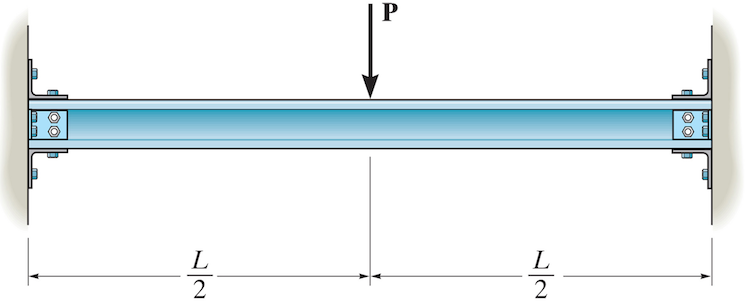
\includegraphics[width=\textwidth]{ch16-reactionmoment}
\end{minipage}
\vspace{-24pt}
\begin{answers}
\correctanswer $1\text{ kN}\cdot\text{m}$
\answer $2\text{ kN}\cdot\text{m}$
\answer $4\text{ kN}\cdot\text{m}$
\answer $8\text{ kN}\cdot\text{m}$
\answer 0
\end{answers}
\begin{solution}
There are multiple equivalent approaches to this problem. We can use superposition to find the constraint moment. There are two options to approach this; one is to include the upward reaction for $P/2$ on the right, and solve for the moment that constrains the slope. The three angle contributions are
\[
\theta(\text{downward force in center}) = -\frac{PL^2}{8EI}
\]
and
\[
\theta(\text{upward force at right constraint}) = +\frac{PL^2}{4EI}
\]
and if a moment $M_0$ is applied at the end, the angle is
\[
\theta(\text{end moment}) = \frac{M_0L}{EI}
\]
The sum is
\[
\begin{split}
-\frac{PL^2}{8EI} + \frac{PL^2}{4EI} + \frac{M_0L}{EI} &= 0\\
\frac{M_0L}{EI} &= -\frac{PL^2}{8EI}\\
M_0 &= -\frac{PL}{8}
\end{split}
\]
Therefore, $M_0 = PL/8 = 1\text{ kN}\cdot\text{m}$.

An alternative approach is to consider and pin-and-ball constrained beam; the end angles would be
\[
\theta = -\frac{PL^2}{16EI}
\]
and if we apply moments $M_0$ at both ends, the angle would be
\[
\theta = -\frac{M_0L}{6EI} - \frac{M_0L}{3EI} = -\frac{M_0L}{2EI}
\]
Then, our constraint is
\[
\begin{split}
-\frac{PL^2}{16EI} - \frac{M_0L}{2EI} &= 0\\
\frac{M_0L}{EI} &= -\frac{PL^2}{8EI}\\
M_0 &= -\frac{PL}{8}
\end{split}
\]
the same as above.

Another approach to this problem is to consider the bending moment diagram, which has slope $P/2$ from $x=0\ldots L/2$ and slope $-P/2$ from $x=L/2\ldots L$. Then,
\[
M(x)=
\begin{cases}
M_0 +\frac{P}{2}x &: x<L/2\\
M_0 -\frac{P}{2}(x-L) &: x>L/2
\end{cases}
\]
If we integrate $M$ from 0 to $L$, we have
\[
\begin{split}
\int_0^L EI\frac{d^2v}{dx^2}\; dx &= \int_0^L M(x)\;dx\\
EI\left.\frac{dv}{dx}\right|_0^L &= M_0 L +\frac{P}{4}\left(\frac{L}{2}\right)^2 +\frac{P}{4}\left(\frac{L}{2}\right)^2\\
0 &= M_0L + \frac{PL^2}{8}
\end{split}
\]
which has the same solution as above.
\end{solution}

\variant
\\
\begin{minipage}[t]{3in}
A $L=4\text{ m}$ beam with constant flexural rigidity $EI$ is fixed to not rotate at each end as shown. What is the magnitude of the reaction moment at either end if the load $P = 4\text{ kN}$?
\end{minipage}
\quad
\begin{minipage}[t]{3in}
\vspace{-12pt}
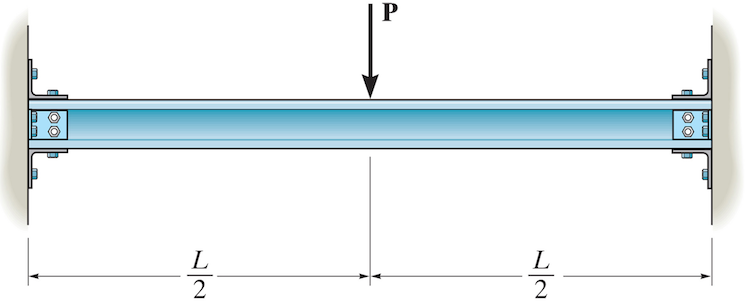
\includegraphics[width=\textwidth]{ch16-reactionmoment}
\end{minipage}
\vspace{-24pt}
\begin{answers}
\correctanswer $2\text{ kN}\cdot\text{m}$
\answer $4\text{ kN}\cdot\text{m}$
\answer $8\text{ kN}\cdot\text{m}$
\answer $16\text{ kN}\cdot\text{m}$
\answer 0
\end{answers}
\begin{solution}
There are multiple equivalent approaches to this problem. We can use superposition to find the constraint moment. There are two options to approach this; one is to include the upward reaction for $P/2$ on the right, and solve for the moment that constrains the slope. The three angle contributions are
\[
\theta(\text{downward force in center}) = -\frac{PL^2}{8EI}
\]
and
\[
\theta(\text{upward force at right constraint}) = +\frac{PL^2}{4EI}
\]
and if a moment $M_0$ is applied at the end, the angle is
\[
\theta(\text{end moment}) = \frac{M_0L}{EI}
\]
The sum is
\[
\begin{split}
-\frac{PL^2}{8EI} + \frac{PL^2}{4EI} + \frac{M_0L}{EI} &= 0\\
\frac{M_0L}{EI} &= -\frac{PL^2}{8EI}\\
M_0 &= -\frac{PL}{8}
\end{split}
\]
Therefore, $M_0 = PL/8 = 2\text{ kN}\cdot\text{m}$.

An alternative approach is to consider and pin-and-ball constrained beam; the end angles would be
\[
\theta = -\frac{PL^2}{16EI}
\]
and if we apply moments $M_0$ at both ends, the angle would be
\[
\theta = -\frac{M_0L}{6EI} - \frac{M_0L}{3EI} = -\frac{M_0L}{2EI}
\]
Then, our constraint is
\[
\begin{split}
-\frac{PL^2}{16EI} - \frac{M_0L}{2EI} &= 0\\
\frac{M_0L}{EI} &= -\frac{PL^2}{8EI}\\
M_0 &= -\frac{PL}{8}
\end{split}
\]
the same as above.

Another approach to this problem is to consider the bending moment diagram, which has slope $P/2$ from $x=0\ldots L/2$ and slope $-P/2$ from $x=L/2\ldots L$. Then,
\[
M(x)=
\begin{cases}
M_0 +\frac{P}{2}x &: x<L/2\\
M_0 -\frac{P}{2}(x-L) &: x>L/2
\end{cases}
\]
If we integrate $M$ from 0 to $L$, we have
\[
\begin{split}
\int_0^L EI\frac{d^2v}{dx^2}\; dx &= \int_0^L M(x)\;dx\\
EI\left.\frac{dv}{dx}\right|_0^L &= M_0 L +\frac{P}{4}\left(\frac{L}{2}\right)^2 +\frac{P}{4}\left(\frac{L}{2}\right)^2\\
0 &= M_0L + \frac{PL^2}{8}
\end{split}
\]
which has the same solution as above.
\end{solution}

\variant
\\
\begin{minipage}[t]{3in}
A $L=4\text{ m}$ beam with constant flexural rigidity $EI$ is fixed to not rotate at each end as shown. What is the magnitude of the reaction moment at either end if the load $P = 2\text{ kN}$?
\end{minipage}
\quad
\begin{minipage}[t]{3in}
\vspace{-12pt}
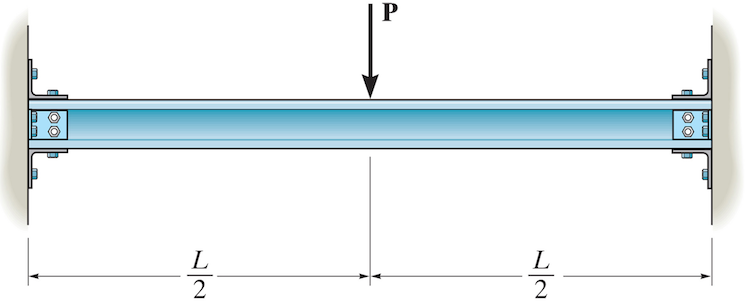
\includegraphics[width=\textwidth]{ch16-reactionmoment}
\end{minipage}
\vspace{-24pt}
\begin{answers}
\correctanswer $1\text{ kN}\cdot\text{m}$
\answer $2\text{ kN}\cdot\text{m}$
\answer $4\text{ kN}\cdot\text{m}$
\answer $8\text{ kN}\cdot\text{m}$
\answer 0
\end{answers}
\begin{solution}
There are multiple equivalent approaches to this problem. We can use superposition to find the constraint moment. There are two options to approach this; one is to include the upward reaction for $P/2$ on the right, and solve for the moment that constrains the slope. The three angle contributions are
\[
\theta(\text{downward force in center}) = -\frac{PL^2}{8EI}
\]
and
\[
\theta(\text{upward force at right constraint}) = +\frac{PL^2}{4EI}
\]
and if a moment $M_0$ is applied at the end, the angle is
\[
\theta(\text{end moment}) = \frac{M_0L}{EI}
\]
The sum is
\[
\begin{split}
-\frac{PL^2}{8EI} + \frac{PL^2}{4EI} + \frac{M_0L}{EI} &= 0\\
\frac{M_0L}{EI} &= -\frac{PL^2}{8EI}\\
M_0 &= -\frac{PL}{8}
\end{split}
\]
Therefore, $M_0 = PL/8 = 1\text{ kN}\cdot\text{m}$.

An alternative approach is to consider and pin-and-ball constrained beam; the end angles would be
\[
\theta = -\frac{PL^2}{16EI}
\]
and if we apply moments $M_0$ at both ends, the angle would be
\[
\theta = -\frac{M_0L}{6EI} - \frac{M_0L}{3EI} = -\frac{M_0L}{2EI}
\]
Then, our constraint is
\[
\begin{split}
-\frac{PL^2}{16EI} - \frac{M_0L}{2EI} &= 0\\
\frac{M_0L}{EI} &= -\frac{PL^2}{8EI}\\
M_0 &= -\frac{PL}{8}
\end{split}
\]
the same as above.

Another approach to this problem is to consider the bending moment diagram, which has slope $P/2$ from $x=0\ldots L/2$ and slope $-P/2$ from $x=L/2\ldots L$. Then,
\[
M(x)=
\begin{cases}
M_0 +\frac{P}{2}x &: x<L/2\\
M_0 -\frac{P}{2}(x-L) &: x>L/2
\end{cases}
\]
If we integrate $M$ from 0 to $L$, we have
\[
\begin{split}
\int_0^L EI\frac{d^2v}{dx^2}\; dx &= \int_0^L M(x)\;dx\\
EI\left.\frac{dv}{dx}\right|_0^L &= M_0 L +\frac{P}{4}\left(\frac{L}{2}\right)^2 +\frac{P}{4}\left(\frac{L}{2}\right)^2\\
0 &= M_0L + \frac{PL^2}{8}
\end{split}
\]
which has the same solution as above.
\end{solution}
